\documentclass[a4paper,12pt]{article} % добавить leqno в [] для нумерации слева

%%% Работа с русским языком
\usepackage{cmap}					% поиск в PDF
\usepackage{mathtext} 				% русские буквы в фомулах
\usepackage[T2A]{fontenc}			% кодировка
\usepackage[utf8]{inputenc}			% кодировка исходного текста
\usepackage[english,russian]{babel}	% локализация и переносы
\usepackage{float}
\usepackage{graphicx}
%%% Дополнительная работа с математикой
\usepackage{amsmath,amsfonts,amssymb,amsthm,mathtools} % AMS
\usepackage{icomma} % "Умная" запятая: $0,2$ --- число, $0, 2$ --- перечисление

%% Номера формул
%\mathtoolsset{showonlyrefs=true} % Показывать номера только у тех формул, на которые есть \eqref{} в тексте.

%% Шрифты
\usepackage{euscript}	 % Шрифт Евклид
\usepackage{mathrsfs} % Красивый матшрифт
\newtheorem{theorem}{Theorem}
\newtheorem{lemma}[theorem]{Lemma}
\theoremstyle{definition}
\newtheorem{definition}{Definition}[section]
%% Свои команды
\DeclareMathOperator{\sgn}{\mathop{sgn}}

%% Перенос знаков в формулах (по Львовскому)
\newcommand*{\hm}[1]{#1\nobreak\discretionary{}
	{\hbox{$\mathsurround=0pt #1$}}{}}

%%% Заголовок
\author{Илья Михеев}
\title{Билеты по Теормеху}
\date{last upd \today  }

\begin{document} % конец преамбулы, начало документа
	
\maketitle 

\section{Скорость и ускорение точки. Естественный трехгранник. Разложение ускорения точки на тангенциальное и нормальное. Криволинейные координаты. Основной и взаимный базисы. Коэффициенты Ламе. Ковариантные и контравариантные компоненты вектора скорости точки в криволинейных координатах. }
\subsection{Скорость и ускорение точки}
 Рассмотрим движение материальной точки $Р$ относительно некоторого тела, которое считается неподвижным.Пусть $О$ --- точка, принадлежащая этому телу. Радиус-вектор $\bf r$ движущейся точки $Р$ относительно $О$ можно задать как вектор-функцию времени: ${\bf r = r}(t)$. С течением времени конец вектора $\bf r$ описывает траекторию точки. Производная от $\bf r$
 \begin{equation}
 	{\bf v}= \frac{d \bf{r}}{d t}
 \end{equation}
называется {\it скоростью точки $P$}. Производной от ${\bf v}$
\begin{equation}
	{\bf w} = \frac{d \bf v}{d t}
\end{equation}
называем {\it ускорением точки $P$}
\subsection{Естественный трехгранник}
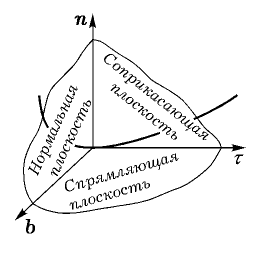
\includegraphics{1_1.png}
Пусть $\sigma (t)$ --- функция длины пути от времени. ${ \tau} (\sigma) = \frac{d \bf \tau}{d \sigma}$ $n = \rho \frac{d \tau}{d t} $ $b = \tau \times n$
\subsection{Разложение ускорения точки на тангенциальное и нормальное}
\begin{equation}
	w = \frac{d^2 \sigma}{d t} \tau + \frac{v_{\tau}^2}{\rho} n 
\end{equation}
\subsection{Криволинейные координаты}

\end{document} % конец документа
